\section*{Les prophètes\footnote{Citation de \textsc{G. Papini}, \textit{Histoire du Christ}, De Fallois 2010, p.~75-77.}}
\decalage « [..]~Le prophète juif est une voix qui parle ou une main qui écrit. Une voix qui parle dans le palais des rois et dans les cavernes des montagnes, sur les marches du Temple et sur les places de la capitale. C'est une voix qui prie, une prière qui menace, une menace qui déborde en divine espérance. Son cœur se consume dans l'affliction, sa bouche est pleine de consternation, son bras se lève pour montrer la punition; il souffre pour son peuple, le couvre de vitupérations parce qu'il l'aime, lui annonce des châtiments pour qu'il se purifie, et par-delà le fer et le feu, enseigne la résurrection et la vie, le triomphe et la béatitude, le règne du nouveau David et le pacte qui ne sera plus révoqué.\par
\decalage «~Le prophète ramène au vrai Dieu les idolâtres, rappelle aux traîtres la foi jurée, aux méchants la charité, aux corrompus la pureté, aux cruels la miséricorde, aux rois la justice, aux rebelles l'obéissance, aux pécheurs le châtiment, aux orgueilleux l'humilité. Il va devant le roi et le gourmande, descend parmi la lie du peuple et la mortifie, s'approche des prêtres et les blâme, se présente devant les riches et les rabroue. Aux pauvres il annonce la consolation, aux affligés la récompense, aux blessés la santé, à la plèbe asservie la libération, au peuple humilié la venue du Vainqueur.\par
\decalage « [..] Le prophète n'est pas philosophe: peu lui importe que le monde soit fait d'eau ou de feu, que l'eau et le feu ne suffisent pas à rendre meilleure l'âme des hommes; il est poète, mais sans le vouloir ni le savoir, quand le trop-plein de l'indignation ou la splendeur du rêve lui mettent dans la bouche des images fortes que jamais les rhéteurs ne sauront inventer; il n'est pas prêtre parce qu'il n'a jamais reçu, dans le Temple, l'onction des gardiens mercenaires des Livres; il n'est pas roi parce qu'il ne commande pas aux armées et n'a d'autre épée que la parole qui vient d'en haut; il n'est pas soldat, mais il est prêt à mourir pour son Dieu et son peuple. \par
\decalage «Le prophète est celui qui voit, le cœur troublé mais l'œil clair, le mal qui règne aujourd'hui, le châtiment qui viendra demain, le règne de félicité qui succédera au châtiment et à la pénitence.\par
\decalage «[..] Le prophète est un accusateur, mais les hommes ne s'avouent pas coupables; un intercesseur, mais les aveugles ne veulent pas que le clairvoyant les prenne par la main; un annonciateur, mais les sourds n'entendent pas ses promesses; un sauveur, mais les moribonds putrides se complaisent dans leur pourriture et refusent d'être sauvés. Et c'est pourtant la parole des prophètes qui témoignera éternellement en faveur de ce peuple qui les extermine mais est aussi capable de les engendrer; et la mort d'un Prophète qui l'emporte sur tous les autres prophètes suffira à expier les crimes de tous les autres peuples qui fouissent la bourbe terrestre.»\par
\vspace{1.5em}
\begin{center}
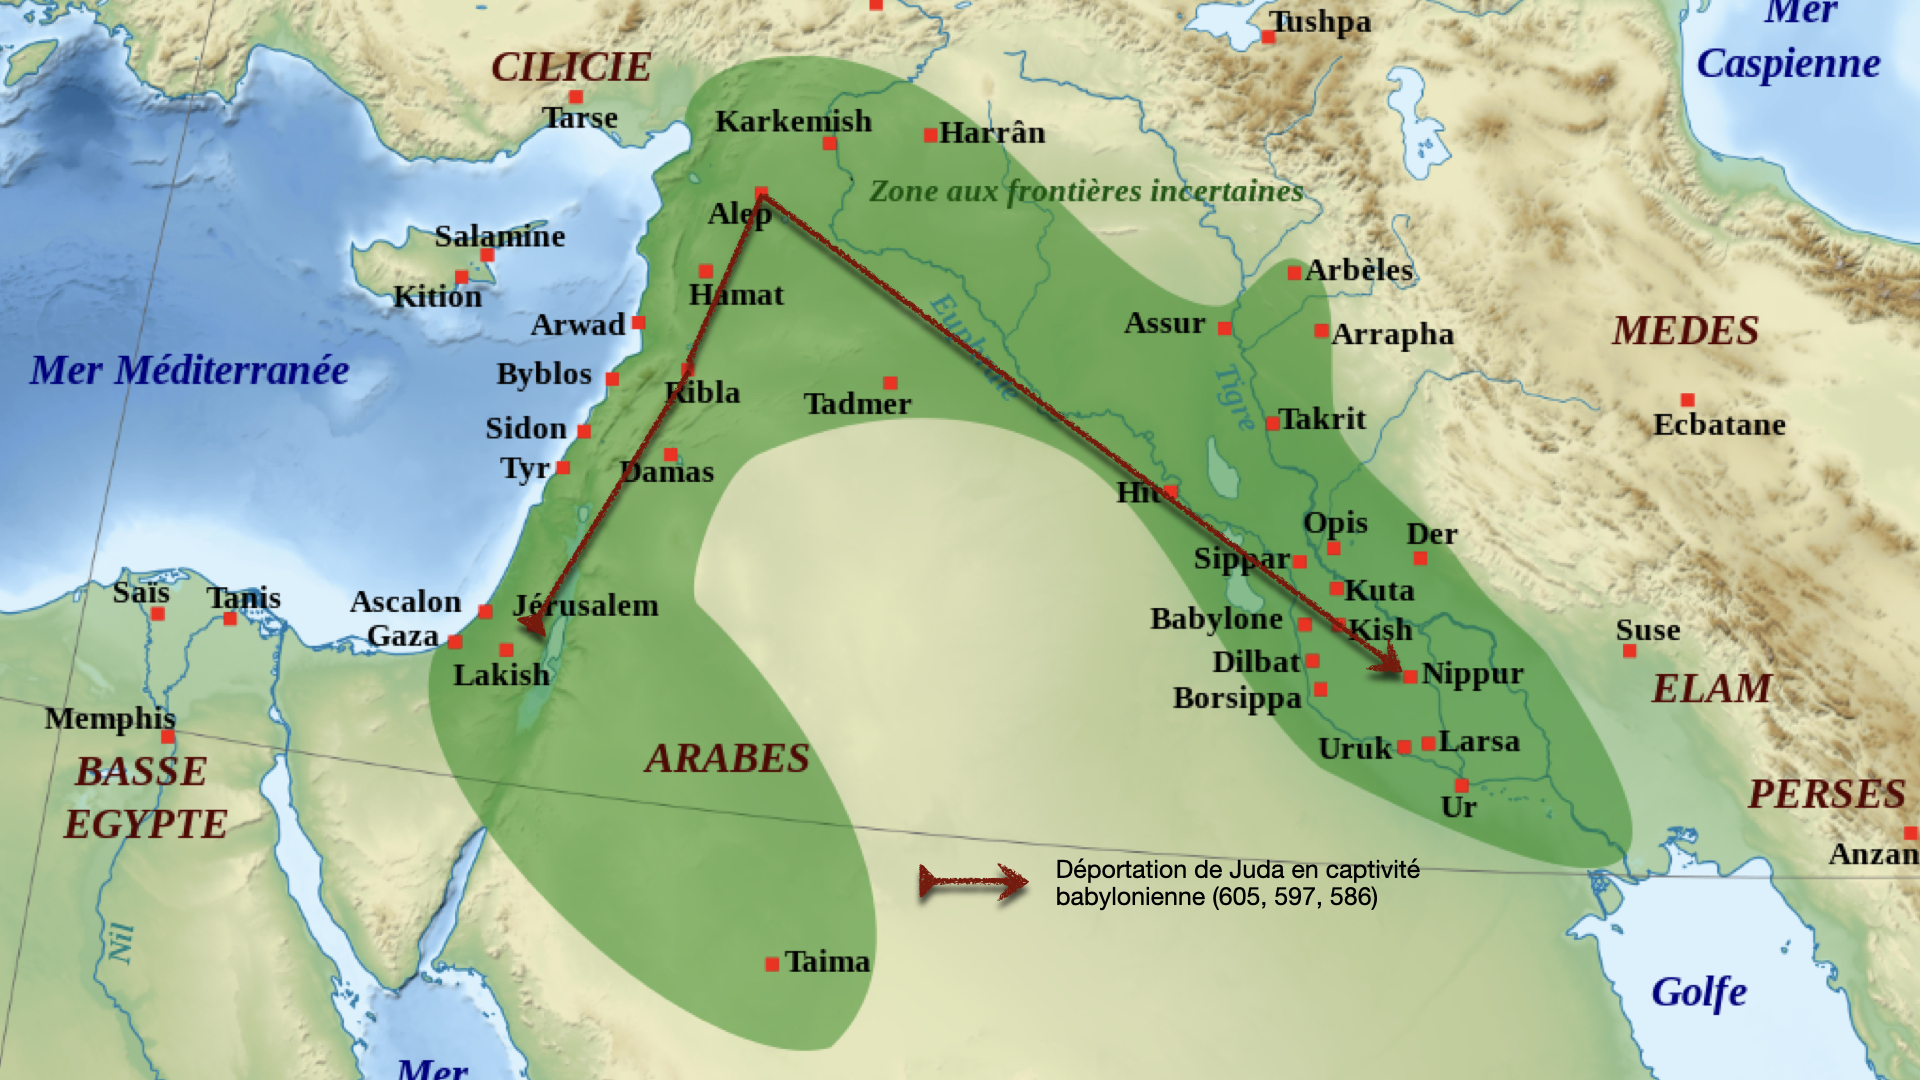
\includegraphics[height=7cm]{../assets/deportation.jpg} \\
\textit{Trajet de la déportation des Juifs de Jérusalem à Babylone}
\end{center}
